\documentclass[UTF8]{ctexart}
%笔者信息
\title{mmWave Sensing 学习笔记}
\author{李东豫  Powered by TI}
\date{\today}
%包引用
\usepackage{amsmath}
\usepackage{graphicx}
\usepackage{enumerate}
%页边距设置
\usepackage{geometry}
\geometry{papersize={210mm,297mm}}
\geometry{left=3cm,right=2.5cm,top=2.5cm,bottom=2.5cm}
\begin{document}
\maketitle
\tableofcontents
\section{概述}
mmWave雷达是近来使用在众多无人驾驶项目中用于建图、避障的高性能传感器,具有分辨率高,不受恶劣天气干扰,隐私性好(想想如果在洗手间安装一个摄像头监控会有多尴尬)的优点。由于开发的需要,我们选择TI的IWR1443毫米波雷达作为载体进行相关学习。
\section{mmWave基础知识}
本节将关注mmWave雷达测量距离、角度、速度的原理进行介绍。
\subsection{什么是FMCW}
\paragraph{FMCW雷达}
的核心是一种称为线性调频脉冲(Chirp)的信号。线性调频脉冲是指雷达信号的频率随时间线性增长的正弦波:f=at,时域波形请见下图\\
{\centering 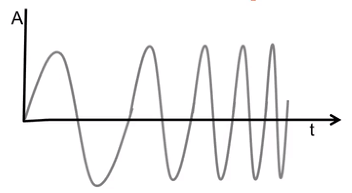
\includegraphics[width = .4\textwidth]{pic/FMCW.png}

}

假设线性调频脉冲以频率$f_c$开始,最终以$f_c+B$的频率结束,那么称B为线性调频脉冲的带宽。因此我们称其为调频连续波,即FMCW。下图为Chirp频域波形:

{\centering 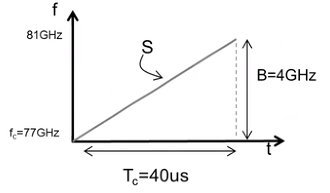
\includegraphics[width = .4\textwidth]{pic/FMCW_Fwave.png}

}

本图例即为IWR1443毫米波雷达的FMCW波形图,其FMCW由初始频率$f_c$,带宽B,以及持续时间$T_c$完全确定。其斜率S决定了线性调频脉冲的频率每单位时间增长的速率。可见在本图中,该线性调频脉冲在40us内扫过了4GHz的带宽,则斜率为100MHz/us.请注意:B和S为定义系统性能的重要参数。

\subsection{FMCW雷达测距原理}
\paragraph{1TX-1RX FMCW雷达}
前方的一个物体会产生一个中频信号(IF Signal)。设雷达信号从TX发射到RX天线接收的时间为τ,则$τ=2d/c$,c为光速,d为雷达与障碍物间距。由此产生的IF信号频率恒定,为$f_{IF}=Sτ=\frac{S2d}{c}.$可推测:雷达前方有多个距离不同的物体时,将产生多个IF信号。该IF信号的频率与距离成正比。

{\centering 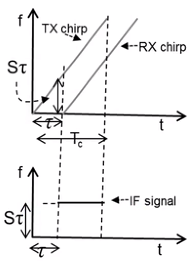
\includegraphics[width = .3\textwidth]{pic/TXRX.png}

}
\subsubsection{mmWave雷达的分辨率与探测距离}
主要是指傅里叶变换对多个距离不同的障碍物所产生的IF信号进行解析时的分辨率。请注意,当两个物体距离过近时,IF信号也会十分接近,进而导致FT无法解析出两个信号的频谱(峰值),进而由频谱混叠导致障碍物数量的误判。
\paragraph{距离分辨率的计算:}

\subparagraph{问题一:}已知一个与雷达相距d的障碍物会使雷达混频器产生频率f=S2d/c的IF信号,且只要两个信号的频率差Δf \textgreater 1/T,那么它们就可以被傅里叶变换分辨(观察时间要大于等于信号的一个周期)。计算雷达的距离分辨率:

{\centering 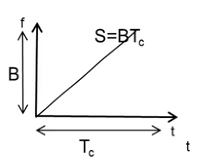
\includegraphics[width = .3\textwidth]{pic/problem_1.png}

}
解:\(\Delta f=\frac{S2\Delta d}{c};\Delta f>\frac{1}{T_c} \),其中$T_c$为IF信号的持续时间\\
请注意此处忽略FMCW一开始的线性调频脉冲的往返时间τ\\
则有:$\frac{S2\Delta d}{c}>\frac{1}{T_c}$\\
可得$\Delta d>\frac{c}{2ST_c}$,且斜率S*线性调频脉冲的持续时间$T_c$等于带宽B\\
∴$\Delta d>\frac{c}{2B},d_{res}=\frac{c}{2B}$\\
\subparagraph{问题二:}如下图所示,若两个雷达的带宽相同,而线性调频脉冲的持续时间不同,哪一个的距离分辨率更好?\\
{\centering 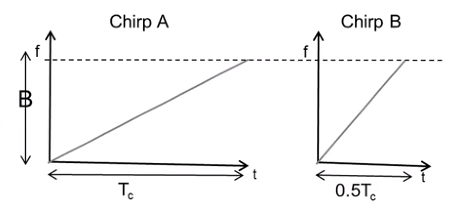
\includegraphics[width = .35\textwidth]{pic/problem_2.png}

}
解:根据问题一所得结果,他们应具有相同的距离分辨率。\\
但Chirp A具有更长的IF信号持续时间,因此具有更长的IF信号观测窗口。因此Chirp A的距离分辨率应优于Chirp B.与问题一矛盾。因此引出IF信号的数字化:
\subparagraph{IF信号的数字化:}有如下几条信息:\\
(1).我们所感兴趣的IF信号的带宽由我们想要的最大探测距离决定:\(f_{IF\_max}=\frac{S2d_{max}}{c}=\frac{2B}{c}\)\\
(2).IF信号通常首先经过低通滤波器,后经过ADC输入至DSP被处理\\
(3).IF带宽因此被ADC采样率$(F_s)$限制.\(F_s >= \frac{S2d_{max}}{c}\)\\
请注意:Nyquist采样定理限定了实信号的采样率应大于等于信号最大频率的2倍,但这里假设基带信号是复信号,因此上式Nyquist采样率为实信号的一半.\\
∴ADC采样率$F_s$限制了雷达的最大探测距离:\(d_{max}=\frac{F_sc}{2S}\)\\
结论:带宽与ADC采样率为影响雷达性能的瓶颈。\\
由于$d_{max}=\frac{F_sc}{2S}$,S与$d_{max}$成正比,可以权衡S与$d_{max}$,设计符合应用目的的雷达。\\
注意:通常雷达倾向于拥有更大的探测距离,因此具有更小的斜率S。

回到问题二上,由于A、B的带宽相同,则它们的距离分辨率相同。但由于Chirp A的斜率S小于Chirp B的斜率,因此对于相同的最大距离要求$d_{max}$,线性调频脉冲A仅需要一半的IF带宽,因此对其进行采样的ADC具有较小的采样率。因此Chirp A的测量时间较长;线性调频脉冲B仅需要一半的测量时间。
\subsubsection{提高mmWave性能方法}
\subparagraph{1:增大IF信号的长度$T_c$},即拓展两个正弦波的观测窗口。请思考这样做可以分开两个频率相近的正弦波信号的原因。请注意:增大观测窗口同时也潜在地增大了带宽,此带宽称为射频带宽(线性调频脉冲的带宽),其范围在几GHz到几百MHz之间。直观上即大带宽对应更好的分辨率。
\subparagraph{2:提高线性调频脉冲频域的斜率S}即增大IF带宽($f_{IF\_max}$),更大的IF带宽等效于更快的线性调频脉冲(即$T_c$更短),更大的最大探测距离$d_{max}$
%Module 2
\subsection{IF信号的相位}
\paragraph{}相位可以响应物体极小的位移,雷达正是基于此原理测量速度的变化。首先提醒一下:在傅里叶变换中,单正弦信号的频谱的峰值的相位对应于正弦波的初始相位。

{\centering 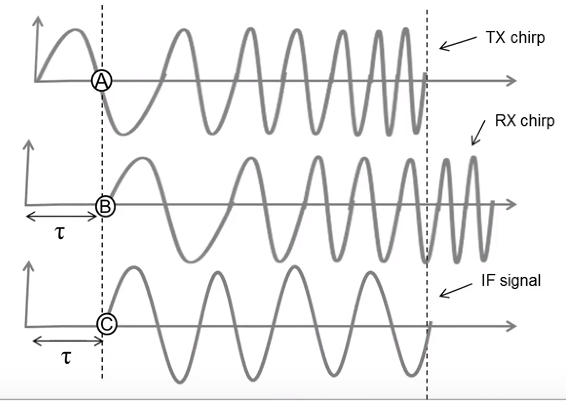
\includegraphics[width = .4\textwidth]{pic/phaseOfIF.png}

}
上图中IF信号为TX、RX经过混频器输出的信号$Asin(2\pi*ft+\phi_0)$,其中频率$f=\frac{S2d}{c}$
\subparagraph{IF信号的相位也会发生相应变化}$\phi_0$=$\phi_A+\phi_B$则当物体移动后,TX-RX发送接收延迟增加Δτ,则此时RX的相位不变,TX相位变化为($\phi_A+2\pi f_c\Delta\tau=\frac{4\pi \Delta d}{\lambda}$)等于IF相位变化。

{\centering 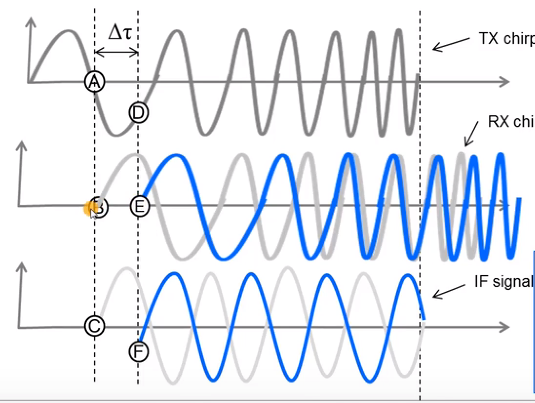
\includegraphics[width = .4\textwidth]{pic/phaseplustau.png}

}

结论:即:IF信号$Asin(2\pi*ft+\phi_0)$的频率随物体间距变化,其起始相位随物体距离的微小变化Δd成线性变化。此处的“微小变化”指相对于雷达的距离分辨率而言的。它必须为若干毫米。\\
\subsubsection{IF信号与物体微小位移的关系}
\paragraph{举例:} 
线性调频脉冲如下图。考虑当雷达前方的物体发生了1mm的位移时,IF信号的变化。(注:对77GHz雷达,1mm=$\lambda/4$)

{\centering 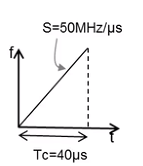
\includegraphics[width = .3\textwidth]{pic/IFsensitivity.png}

}

解:由前面推导:IF信号的相位变化$\Delta \phi=\frac{4 \pi \Delta d}{\lambda}=\pi=180^\circ$\\
IF信号的频率变化$\Delta f=\frac{S2\Delta d}{c}=333Hz$\\
对于观察窗口$T_c=40us$,$\Delta f$对应周期数目为$\Delta f T_c=333*40*10^-6=0.013 cycles$,如此微小的变化在FFT中体现不出来。\\
结论:IF信号的相位对物体距离的微小变化量十分敏感,而频率对其不敏感。
\subsubsection{用两个线性调频脉冲测量物体速度v}

{\centering 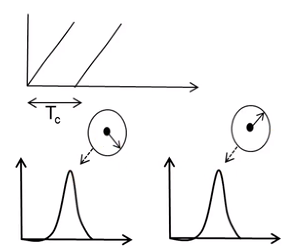
\includegraphics[width = .4\textwidth]{pic/speedmes.png}

}

\paragraph{}以$T_c$为时间间隔发送两个线性调频脉冲,对得到的IF信号进行FFT运算,他们将有相同的峰值但相位不同。测得的相位差$\omega$对应于物体的运动$vT_c$。\\
\[\omega=\frac{4\pi v T_c}{\lambda} ,v=\frac{\lambda \omega}{4\pi T_c}\]



由上式,可知$\Delta \phi$与$\Delta d$成正比,$\Delta \phi$的变化周期T也直接反映了震动周期。

{\centering 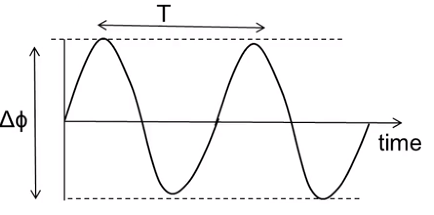
\includegraphics[width = .4\textwidth]{pic/deltaphase.png}

}

\subparagraph{补充}:\\
(1) 由于mmWave雷达对于微小振动敏感,因此也常用来作为电机振动监测、心跳检测等应用的核心部件。\\
(2) 当有多个物体恰好与雷达的距离相同,但拥有不同的移动速度。那么距离FFT(Range FFT,即上文中使用的FFT)将只输出单个与此距离d对应的峰值。分离方法:多普勒FFT:用于分离多个距离相同但速度不同的物体。
%Module 3
\subsection{速度估计}
\paragraph{FFT}与一个相量以恒定离散角速度$\omega$(/次采样)的速率旋转(即每两个样本之间相隔$\omega$弧度),其FFT将在$\omega$处产生一个峰值
\subparagraph{分辨率的问题:}
当一个信号内由两个相量构成时,FFT理应有$\omega_1$与$\omega_2$两个峰值。\\
请注意:输入序列的长度越长,FFT的分辨率越高。一般地,一个长度为N的序列可以分辨两个角速度差大于$2\pi/N$的信号。
\subparagraph{比较连续信号与离散信号的分辨率}:\\
	连续信号:$\Delta f=\frac{1}{T} (cycles/sec)$,其中T为观察窗口\\
	离散信号:$\Delta \omega=\frac{2\pi}{N}(rad/sample) = \frac{1}{N} (cycles/sample)$,N为观测样本数
\subparagraph{最大可测量速度}与波长和观察时间有关。当物体远离雷达向远处移动时,$\omega>0$;当物体远离雷达向近处移动时,$\omega<0$。考虑$e^{j\omega}$周期为2π,当$|\omega|>180^\circ=\pi$时,将无法判断物体的运动方向。即:\\
不产生歧义的速度测量:$|\omega|<\pi$\\
∴$\frac{4\pi v T_c}{\lambda}<\pi$,即$v<\frac{\lambda}{4T_c}$\\
得到:\[v_{max}=\frac{\lambda}{4T_c}\]其中$T_c$为两个Chirp间隔。\\
因此要得到更高的最大可测量速度,需要由更密集的线性调频脉冲(降低$T_c$)

\subsubsection{测量距离相同的多个物体的速度}
\paragraph{考虑}两个与雷达相距均为d,但速度分别为$v_1,v_2$,它们均向雷达靠近。
由于距离相同,Range-FFT的输出将只有一个峰值,但峰值处的相量相位将具有两个物体的分量。
\paragraph{解决方案}:
\subparagraph{发射一系列等间隔的线性调频脉冲},而不仅仅是两个Chirps.假设发射N个Chirps(通常称它们为1帧),对一系列相量做Range-FFT,得到的一组Range-FFT总会在相同的位置有一个峰值,但与这些相量相对应的离散序列有两个旋转相量,分别为$\omega_1,\omega_2$,对应$v_1,v_2$。因此对这个序列的FFT将有两个峰值$\omega_1,\omega_2$。将其代入下式,得到两物体的速度:\\
\[v_1=\frac{\lambda \omega_1}{4 \pi T_c}\]
\[v_2=\frac{\lambda \omega_2}{4 \pi T_c}\]\\
请注意:这里的FFT是在线性调频脉冲之间执行的,通常称为多普勒FFT(doppler-FFT)。
\subparagraph{多普勒FFT的速度分辨率},即$v_1,v_2$之间的最小间隔可由以下条件给出:\\
两个物体的速度差为$\Delta v$,则其角频率差为\(\Delta \omega=\frac{4\pi \Delta v T_c}{\lambda}\)\\
对于序列长度为N的FFT,当其角频率差值$\Delta \omega>\frac{2\pi}{N}$时,可被FFT分辨。\\
∴$\frac{4\pi \Delta v T_c}{\lambda}>\frac{2\pi}{N}$,即$\Delta v > \frac{\lambda}{2NT_c}$\\
即$v_{res}=\frac{\lambda}{2NT_c}=\frac{\lambda}{2T_f}$,$T_f$为帧时间长度。\\
\subparagraph{问题:}两个雷达的帧如下

{\centering 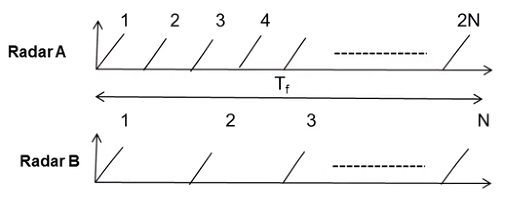
\includegraphics[width = .4\textwidth]{pic/diffframe.png}

}
问:如何评价两个雷达的最大测量速度$v_{max}$与速度测量精度$v_{res}$?\\
答:两个雷达的帧时间长度相同,且FMCW的带宽相同、斜率S相同。则$\lambda$相同\\
∴$v_{res}=\frac{\lambda}{2T_f}$,可得两个雷达速度测量精度$v_{res}$相同。\\
由$v_{max}=\frac{\lambda}{4T_c}$,其中$T_c$为两个Chirps之间的时间间隔,可知Radar A的最大可测量速度较大。

%Module 4
\subsection{设计mmWave雷达系统}
本节主要目标位设计一个符合制定标准(速度分辨率,最大测量速度等),并粗略了解一些更深层的雷达设计知识。
\subsubsection{回顾FMCW 2D FFT处理}
首先,可以使用距离FFT(Range-FFT)来解析处于不同距离的物体,然后,多普勒FFT(doppler-FFT)对一帧中的后续的线性调频脉冲进行解析,可以解析出处于距离相近但速度不同的物体。
\paragraph{梳理}:\\
(1)雷达Tx天线发射一系列时间间隔相同的线性调频脉冲,称为一帧。\\
(2)雷达Rx端对接收的信号进行ADC采样。请注意:ADC采样得到的数据将是连续不断的,前一个线性调频脉冲对后一个Chirp进行影响的数据。(请好好理解)\\
(3)DSP或其他处理器对ADC采得的数据,即距离单元进行距离FFT(对每一个单独的线性调频脉冲--此时的线性调频脉冲由于受到前一个脉冲的叠加,因此改称为range-bin,距离单元),得到物体之间的距离\\
(4)DSP再对所有距离单元进行多普勒FFT,得到距离相近物体的不同速度(注意是所有!因此多普勒FFT必须在一帧全部接收后才能进行)。\\
说明:DSP在接收到数据时以“内联”方式对ADC数据进行距离FFT,之后将距离FFT数据存储到存储单元中——距离单元。ADC数据不被储存。之后对其进行多普勒FFT。此操作称为2维FFT。
\subparagraph{公式回顾}:\\
\[v_{max}=\frac{\lambda}{4T_c},v_{res}=\frac{\lambda}{2T_f}\]
\[d_{res}=\frac{c}{2B}\]
\[F_{if\_max}=\frac{S2d_{max}}{c}\]
\subsubsection{系统设计}
\paragraph{考虑:}给定距离分辨率$d_{res}$,最大距离$d_{max}$,速度分辨率$v_{res}$,最大可测量速度$v_{max}$,如何设计一帧?
\subparagraph{}
可能的解法:\\
(1)首先从$v_{max}$开始,由上公式可见$v_{max}$仅取决于$T_c$,即线性调频脉冲之间的时间间隔。因此,给定$v_{max}$,直接可得:
\[T_c=\frac{\lambda}{4v_{max}}\]
(2)注意到距离分辨率$d_{res}$仅取决于线性调频脉宽的带宽B,因此可求得:
\[B=\frac{c}{2d_{res}}\]
请注意,此时由于$T_c$与B均已确定,则Chirps的斜率S也已锁定。\\
(3)速度分辨率$v_{res}$仅取决于一帧的时间$T_f$,因此可求得:
\[T_f=\frac{lambda}{2v_{res}}\]
此时整个帧的定义就结束了。但这整个过程没有用到第四个方程。更详细的讨论将在下面给出。
{\centering 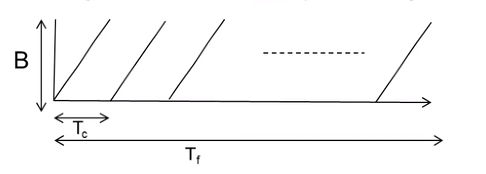
\includegraphics[width = .4\textwidth]{pic/defineaframe.png}

}

在实际开发中,设定线性调频脉冲的参数的过程可能比上面的讨论更有'迭代性'。比如:
\begin{enumerate}[1)]
\item [1)]
设备可能不支持所需的最大IF带宽:由于\(F_{if\_max}=\frac{S2d_{max}}{c}\),设计者需要按需平衡S或$d_{max}$。
\item [2)]
设备在发射调频脉冲时必须能够生成所需的斜率S(通常雷达中的合成器对能够生成的最大斜率有限制)。
\item [3)]
调频脉冲之间的空闲时间$T_c$可能存在于特定设备的要求。
\item [4)]
设备必须有足够大的内存来存储所有脉冲的距离FFT数据,否则多普勒FFT无法进行。
\end{enumerate}
\subparagraph{S与$d_{max}$的取舍}
由公式可知:$d_{max}$增加对应着S必须减小。假设脉冲的时间长度$T_c$一定($T_c$由$v_{max}$决定),当斜率S降低时会直接导致带宽B降低,从而导致距离分辨率$d_{res}$降低。
{\centering 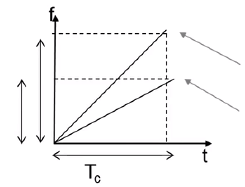
\includegraphics[width = .4\textwidth]{pic/sdconflicts.png}

}

通常的做法是:对于给定的脉冲时间$T_c$:
\begin{enumerate}[1)]
\item [1)]
一个短距离雷达会提高斜率S,从而有更大的带宽$->$更好的距离分辨率
\item [2)]
一个长距离雷达会降低斜率S,从而有较小的带宽。
\end{enumerate}
\subsubsection{雷达距离方程}
\paragraph{影响雷达最大探测距离的其他因素}
当雷达发射脉冲后,该最大距离物体反射的信号应该有足够的强度才能被雷达接收到。

{\centering 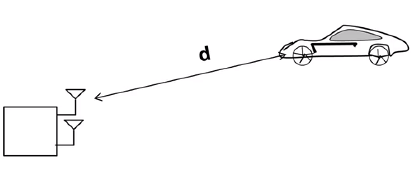
\includegraphics[width = .4\textwidth]{pic/POWER.png}

}
如图所示,雷达发射输出功率为$P_t$,由于信号被不断地扩散,其功率密度随距离d的平方成反比,即:

{\centering
\qquad发射功率密度=\(\frac{P_tG_{TX}}{4\pi d^2}\)$W/m^2$\\
}

可以通过使用更高功率增益的天线来提高功率密度,其工作方式通常是通过提高方向性来束缚功率扩散。上式中的$G_TX/RX$即天线的发射/接收增益。此时被物体反射的功率密度为

{\centering
发射功率密度*$\sigma$=\(\frac{P_tG_{TX}\sigma}{4\pi d^2}\)W\\}
其中$\sigma$为目标的雷达截面积(Radar Cross Section,RCS),用于表示雷达接收端方向上反射雷达信号的强度。

因而可推出雷达接收天线处的功率密度为:
\[\frac{P_tG_{TX}\sigma}{(4\pi)^2 d^4}\]\\
雷达RX天线捕获到的功率为
\[P_{capture}=
\frac{P_tG_{TX}\sigma A_{RX}}{(4\pi)^2 d^4}=
\frac{P_tG_{TX}\sigma G_{RX}\lambda^2}{(4\pi)^3 d^4}
\]\\
$A_{RX}$为RX天线的有效孔径面积,度量了天线捕获接收信号的能力:\(A_{RX}=\frac{G_{RX}\lambda^2}{4\pi}\)\\
另外还有一件重要的事实:接收信号中会混有噪声。噪声太大会直接淹没原信号,所以这里我们需要用到信噪比SNR的概念:SNR=信号功率/噪声功率。在雷达中,有
\[SNR=\frac{\sigma P_tG_{TX}G_{RX}\lambda^2 T_{meas}}{(4\pi)^3 d^4 kTF}\]
其中$T_{meas}$为总测量时间:$T_{meas}=NT_c$,k为玻尔兹曼常数,T为天线温度(绝对温度)。kTF为接收端的热噪声\\
当雷达检测一个物体时,对SNR最小值有限制:$SNR_{min}$的典型值为15dB-20dB。当接收到的SNR低于最小SNR时,任何目标将不被视为有效目标。\\
给定$SNR_{min}$,可计算雷达最大探测距离:
\[d_{max}=(\frac{\sigma P_tG_{TX}G_{RX}\lambda^2 T_{meas}}{(4\pi)^3 SNR_{min} kTF})^{\frac{1}{4}}\]

\subsection{角度估计}

{\centering 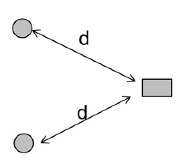
\includegraphics[width = .3\textwidth]{pic/angleestimate.png}

}

考虑一个问题:当有两个物体雷达的距离与速度均相同时,如何分辨二者?此时多普勒FFT与距离FFT均已不能分辨。本小节主要介绍使用多个天线来估计物体的到达角(Angle of arrival)的方法。

\paragraph{到达角(A0A)测量基础}:
复习:当物体在距离上改变一个微小量$\Delta d$之后,距离FFT的峰值处将会产生一个相位变化。

{\centering 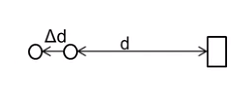
\includegraphics[width = .3\textwidth]{pic/angleest.png}

}

\[\Delta \omega=\frac{4\pi \Delta d}{\lambda}\]
\paragraph{}
角度估计使用了类似的原理。角度估计需要至少两个RX天线,物体距离两个天线的距离差将会导致2D-FFT中峰值的相位变化,由此计算AoA。

{\centering 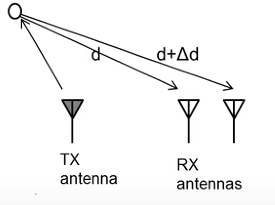
\includegraphics[width = .3\textwidth]{pic/twoRX.png}

}

同理,\(\Delta \omega=\frac{2\pi \Delta d}{\lambda}\),请注意上式中$2\pi$的因子项。
\subsubsection{具体过程分析}
\begin{enumerate}[1)]
\item [1)]
TX天线发射一帧线性调频脉冲
\item [2)]
每个RX天线进行2D-FFT,他们将在同一个位置有峰值,但相位不同
\item [3)]
测量的相位差$\Delta \omega$可以用于测量AoA
\end{enumerate}
{\centering 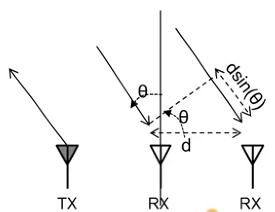
\includegraphics[width = .3\textwidth]{pic/analysis.png}

}

上图中d为两个RX天线之间的距离,假设物体离两天线距离足够远,则两条反射波平行,$\theta$时物体相对于雷达的到达角,则有:
\[\omega=\frac{2\pi d sin(\theta)}{\lambda} \, -> \, \theta=sin^{-1}(\frac{\lambda \omega}{2\pi d})\]
可见$\omega$与$\theta$为非线性关系,在$\theta =0$时,$\omega$对$\theta$的变化最为敏感,当$\theta$增加时,角度估计误差更容易出现误差。

{\centering 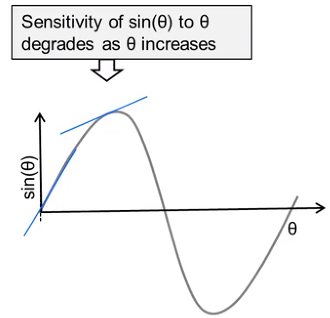
\includegraphics[width = .3\textwidth]{pic/sensitivety.png}

}
{\centering 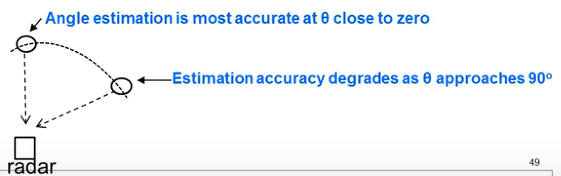
\includegraphics[width = .7\textwidth]{pic/thetasens.png}

}

\subsubsection{雷达的最大视场}
\paragraph{}与最大可测量速度类似,雷达左侧的物体与雷达右边的物体之间的$|\Delta \omega|<180^{\circ}$,否则无法判断。\\
\[=> \frac{2\pi d sin(\theta)}{\lambda}<\pi=>\theta<sin^{-1}(\frac{\lambda}{2d})\]
可推出雷达RX天线相距为d,则最大视场为\(\theta_{max}=sin^{-1}(\frac{\lambda}{2d})\)\\
相距为$\frac{\lambda}{2}$的雷达可以得到最大视场$+-90^{\circ}$\\
\subsubsection{测量具有相同距离与速度的两个物体}
{\centering 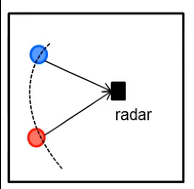
\includegraphics[width = .2\textwidth]{pic/sametwo.png}

}

\paragraph{}
由于两个物体具有相同的位置,则距离FFT的峰值位置相同;相同的速度导致多普勒FFT峰值相同。但当使用两个RX天线时,两个RX天线进行FFT的相量的相位将不会相同。\\
因此,解决方案:使用N组接收天线的矩阵。对这N组RX天线的2D-FFT进行再次FFT,将会解析两个物体。称为角度FFT(angle-FFT)。

{\centering 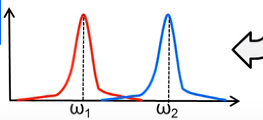
\includegraphics[width = .3\textwidth]{pic/angleFFT.png}

}

$\omega_1$ 和$\omega_2$ 对应于两个连续的线性调频脉冲的相位差(两个物体),反向计算可得两物体的AoA$=> \theta_x=sin^{-1}(\frac{\lambda \omega_x}{2\pi d})$,其中x为1,2

\subsubsection{角度分辨率}
\paragraph{}
当两个物体之间的夹角小于$\Delta \theta$时,将无法分辨物体个数。此$\Delta \theta$称为角度分辨率。
\subparagraph{解算方法}:\\
(1)两物体相隔$\theta$角时,其角度FFT计算出的离散频率为$\omega=\frac{2\pi d sin(\theta)}{\lambda}$\\
(2)频域可分辨的标准:$\Delta \omega > \frac{2\pi}{N}$,N为FFT的样本数(在这里是天线的个数)\\
可解出

{\centering 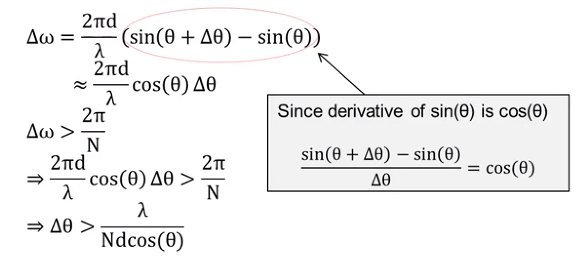
\includegraphics[width = .7\textwidth]{pic/result.png}

}

\end{document}

